% !TeX spellcheck = ru_RU
% !TEX root = vkr.tex

\section{Экспериментальное исследование}

\subsection{Методология эксперимента}

Эксперименты проводились на трёх платформах. Banana Pi BPI-F3 оснащён процессором SpacemiT K1 (8 ядер RISC-V @ 2.0 ГГц), GPU IMG BXE-2-32 и 16 ГБ LPDDR4-2666. StarFive VisionFive 2 использует процессор JH7110 (4 ядра RISC-V @ 1.5 ГГц), GPU IMG BXE-4-32 MC1 и 8 ГБ LPDDR4-2800. Intel Core i9-12900H имеет 14 ядер (до 5.0 ГГц), Intel Iris Xe Graphics и 24 ГБ DDR5-4800.

Для автоматизации тестирования использовался репозиторий matrix-benchmark~\cite{matrix_benchmark_repo} со скриптами \texttt{benchmark.sh} и \texttt{conf.sh}. Библиотека CLBlast тестировалась в двух вариантах: со стандартными параметрами и после автоматического тюнинга встроенной утилитой \texttt{clblast\_tuner\_xgemm}.

Для MyGEMM выполнялось по 100 прогонов каждой конфигурации, для CLBlast --- по 10 прогонов. Измерялось только время выполнения OpenCL ядра без учёта загрузки данных. Основной размер матриц для сравнения --- $1024 \times 1024$ элементов типа \texttt{float}, для анализа масштабируемости CLBlast использовался диапазон от $512 \times 512$ до $7680 \times 7680$. Стандартное отклонение измерений не превысило 2\% для всех конфигураций.

\subsection{Тестирование библиотеки MyGEMM}

При первом запуске библиотеки MyGEMM~\cite{mygemm_repo} возникла ошибка выполнения OpenCL ядер. Сообщение об ошибке указывало на проблему с созданием рабочих групп (work-groups), однако точная причина не была очевидна.

Для выяснения причины был проанализирован исходный код библиотеки. Изучение реализации различных ядер показало, что ключевыми параметрами, определяющими размер рабочих групп, являются константы TS (Tile Size), TSM (Tile Size M) и TSN (Tile Size N). Согласно документации MyGEMM~\cite{nugteren2018mygemm}, эти параметры определяют размерность блоков данных, обрабатываемых одной рабочей группой. Для ядер 1--3 размер рабочей группы составляет $\text{TS} \times \text{TS}$ потоков, для ядер 4--10 размер определяется как $\frac{\text{TSM}}{\text{WPTM}} \times \frac{\text{TSN}}{\text{WPTN}}$ потоков.

Значения по умолчанию в библиотеке установлены для дискретных GPU NVIDIA. Для ядер 1--3 используется TS = 32, что создаёт рабочие группы размером $32 \times 32 = 1024$ потока. Для ядер 6--10 используются TSM = 128, TSN = 128, WPTM = 8, WPTN = 8, что даёт размер группы $\frac{128}{8} \times \frac{128}{8} = 16 \times 16 = 256$ потоков.

Для определения аппаратных ограничений платформ была использована утилита \texttt{clinfo}~\cite{clinfo}. Анализ вывода утилиты на обеих платформах показал, что максимальный размер рабочей группы (параметр \texttt{CL\_DEVICE\_MAX\_WORK\_GROUP\_SIZE}) составляет 512 потоков. Это существенно отличается от типичных значений для дискретных GPU (1024--2048 потоков), что объясняет ошибку при запуске с параметрами по умолчанию: размер группы 1024 потока превышает аппаратное ограничение.

С учётом выявленного ограничения были модифицированы параметры запуска для всех ядер библиотеки. Для ядер 1--3 параметр TS был установлен в значения 8 и 16, что даёт размеры рабочих групп 64 и 256 потоков соответственно. Для ядер 4--10 были подобраны комбинации параметров TSM и TSN из множества \{32, 64, 128\} с соответствующими значениями WPTM и WPTN, обеспечивающие соблюдение ограничения на размер рабочей группы. После внесения изменений библиотека успешно запустилась на обеих платформах, что позволило перейти к исследованию производительности различных ядер.

Для тестирования использовались 11 реализаций ядра MyGEMM с параметрами, адаптированными под ограничение размера рабочей группы для RISC-V платформ. Ядра 1--2 тестировались с параметром TS со значениями 8 и 16 (значение 32 вызывало ошибку \texttt{Invalid work group size}). Ядро 3 тестировалось с параметрами TS 8, 16, 32. Для ядер 4--10 использовались комбинации параметров TSM и TSN из множества \{32, 64, 128\} с соответствующими значениями WPTM и WPTN, всего 9 конфигураций для каждого ядра. Оптимизация, соответствующая оптимизации 11, тестировалось с фиксированной конфигурацией из реализации clBLAS.

Результаты представлены на рисунках~\ref{fig:perf_bananapi}--\ref{fig:perf_intelxe}. Производительность существенно различается между платформами: Intel выполняет операции за 0.004--0.029 секунд, Banana Pi --- за 0.3--11 секунд (в 75--380 раз медленнее), StarFive --- за 0.5--9 секунд (в 125--225 раз медленнее).

\begin{figure}[H]
\centering
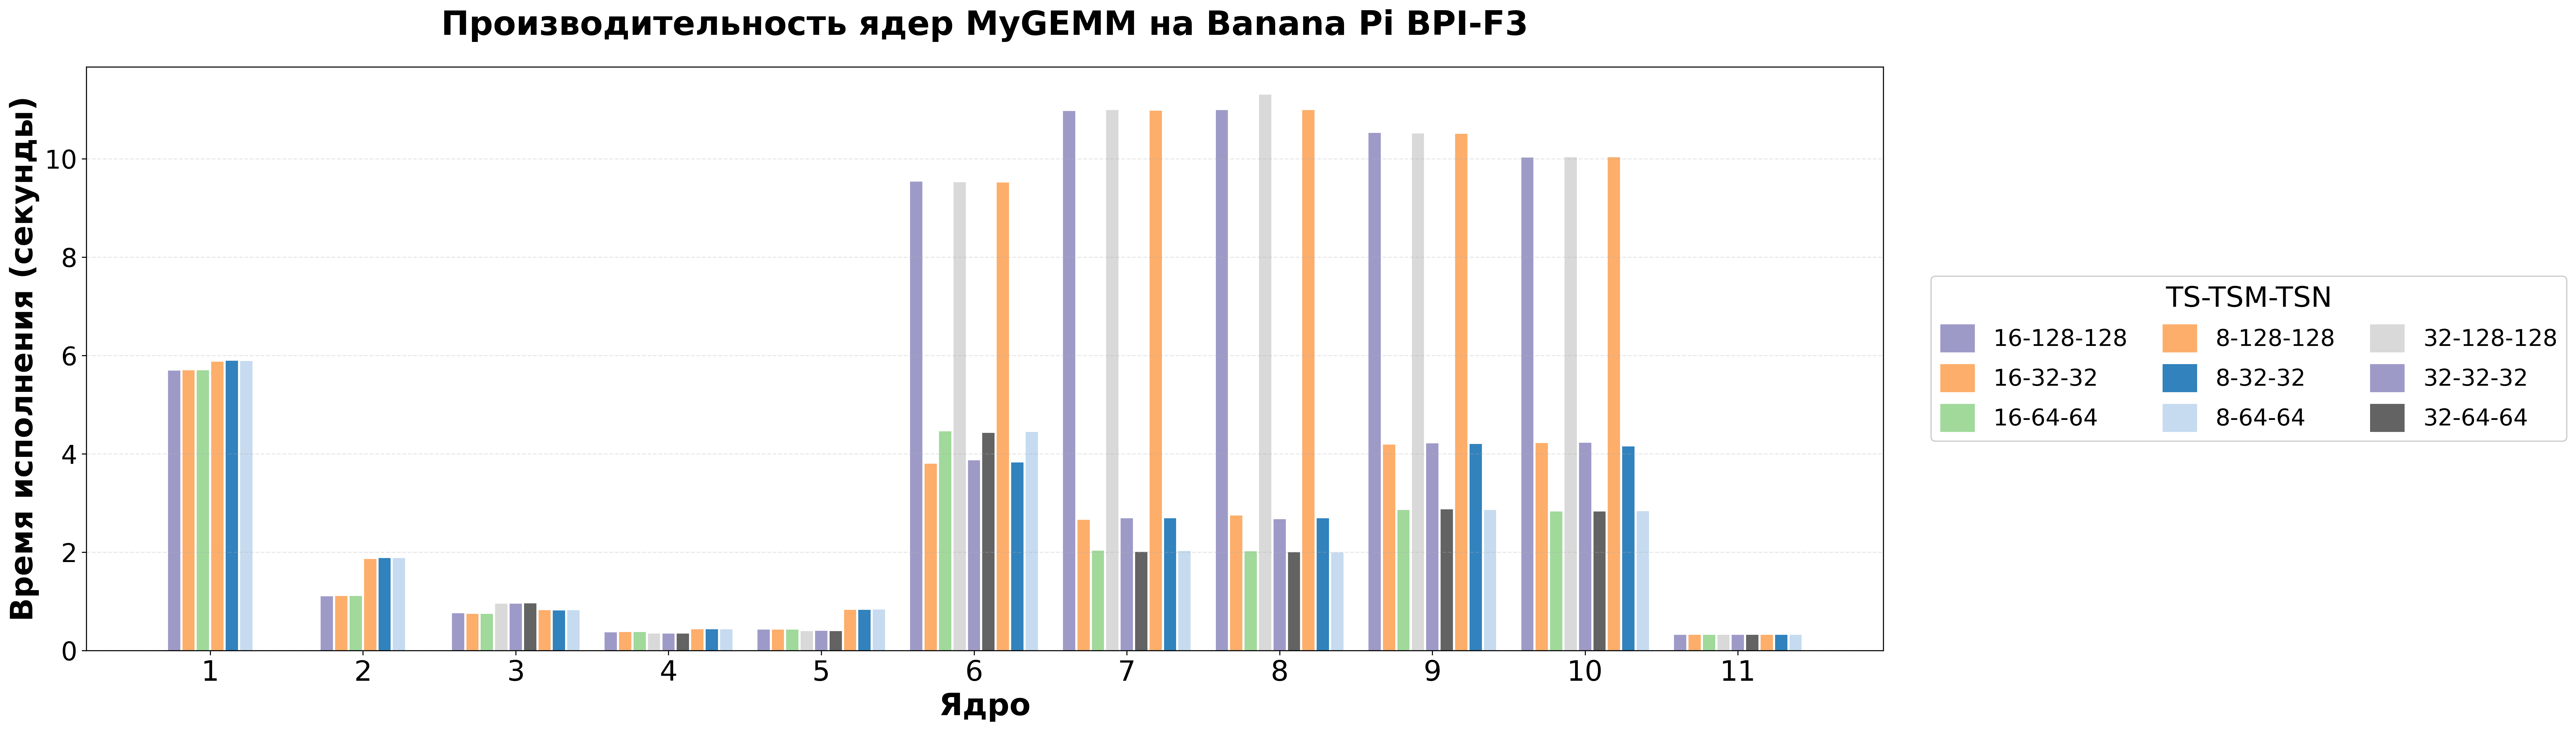
\includegraphics[width=1\textwidth]{figures/banana_pi.png}
\caption{Производительность ядер MyGEMM на платформе Banana Pi BPI-F3}
\label{fig:perf_bananapi}
\end{figure}

\begin{figure}[H]
\centering
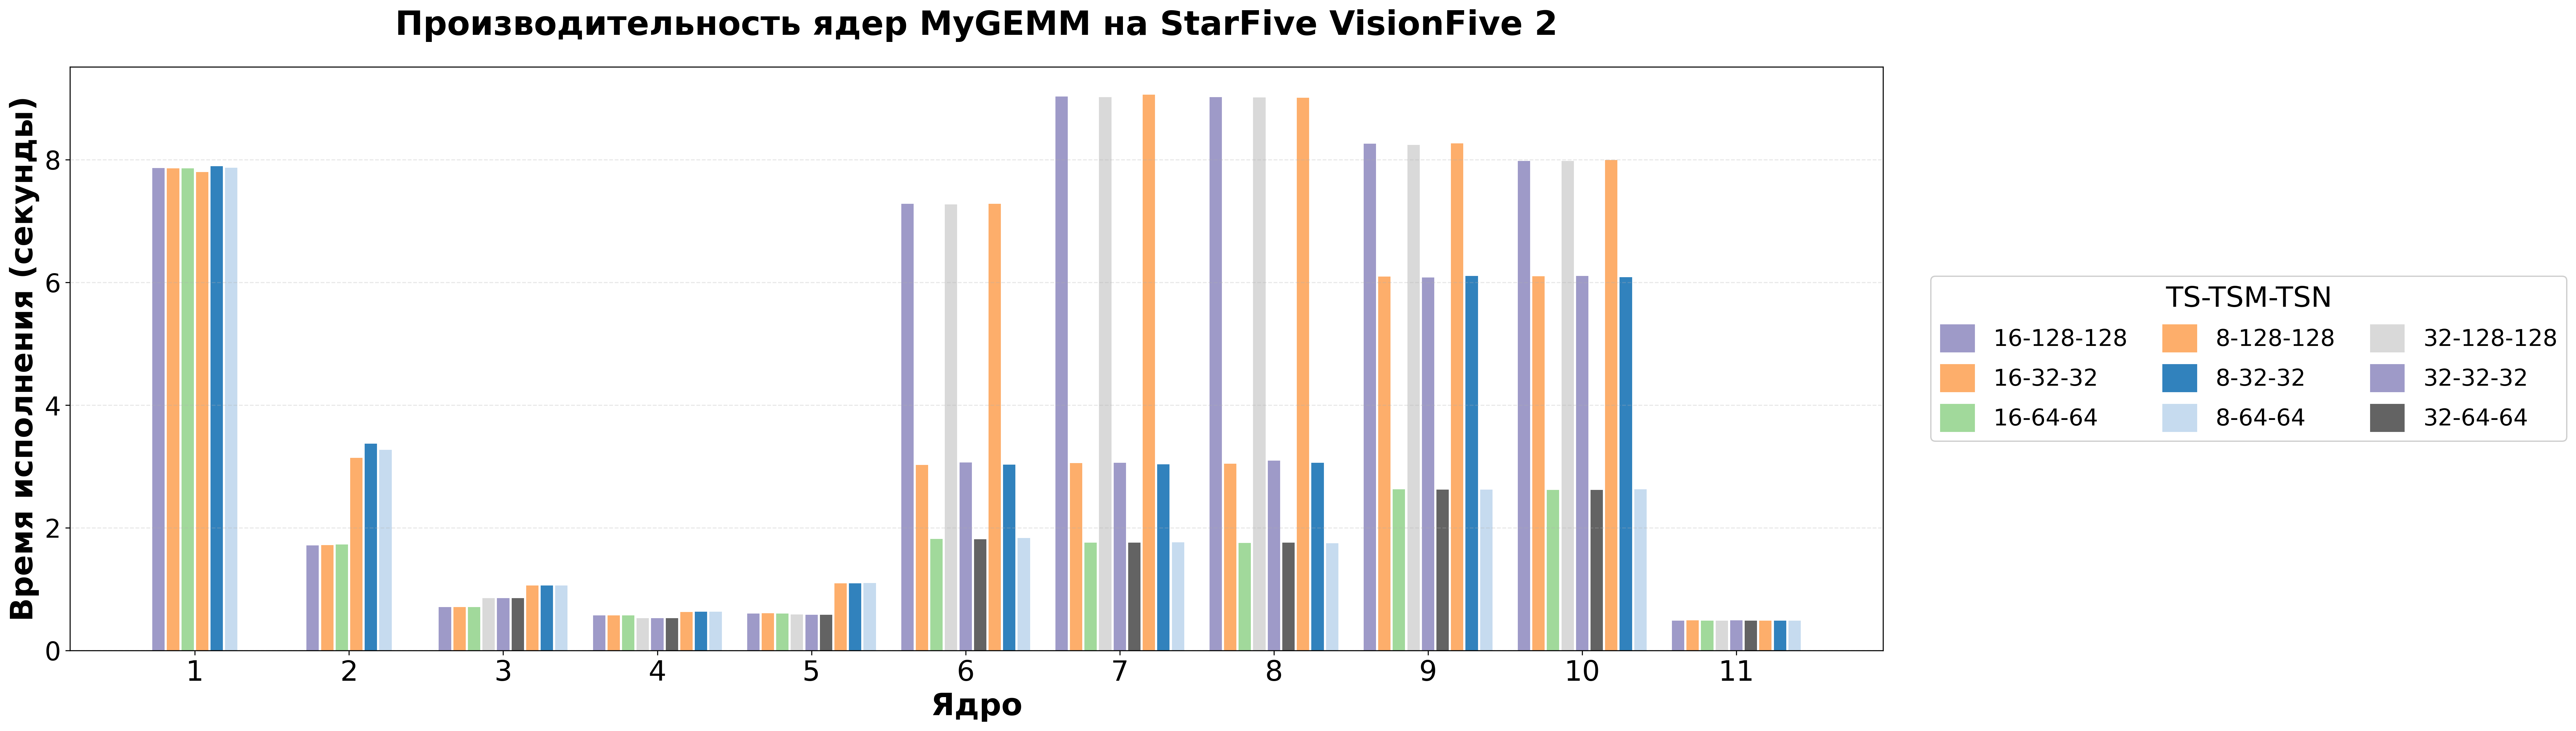
\includegraphics[width=1\textwidth]{figures/starfive.png}
\caption{Производительность ядер MyGEMM на платформе StarFive VisionFive 2}
\label{fig:perf_starfive}
\end{figure}

\begin{figure}[H]
\centering
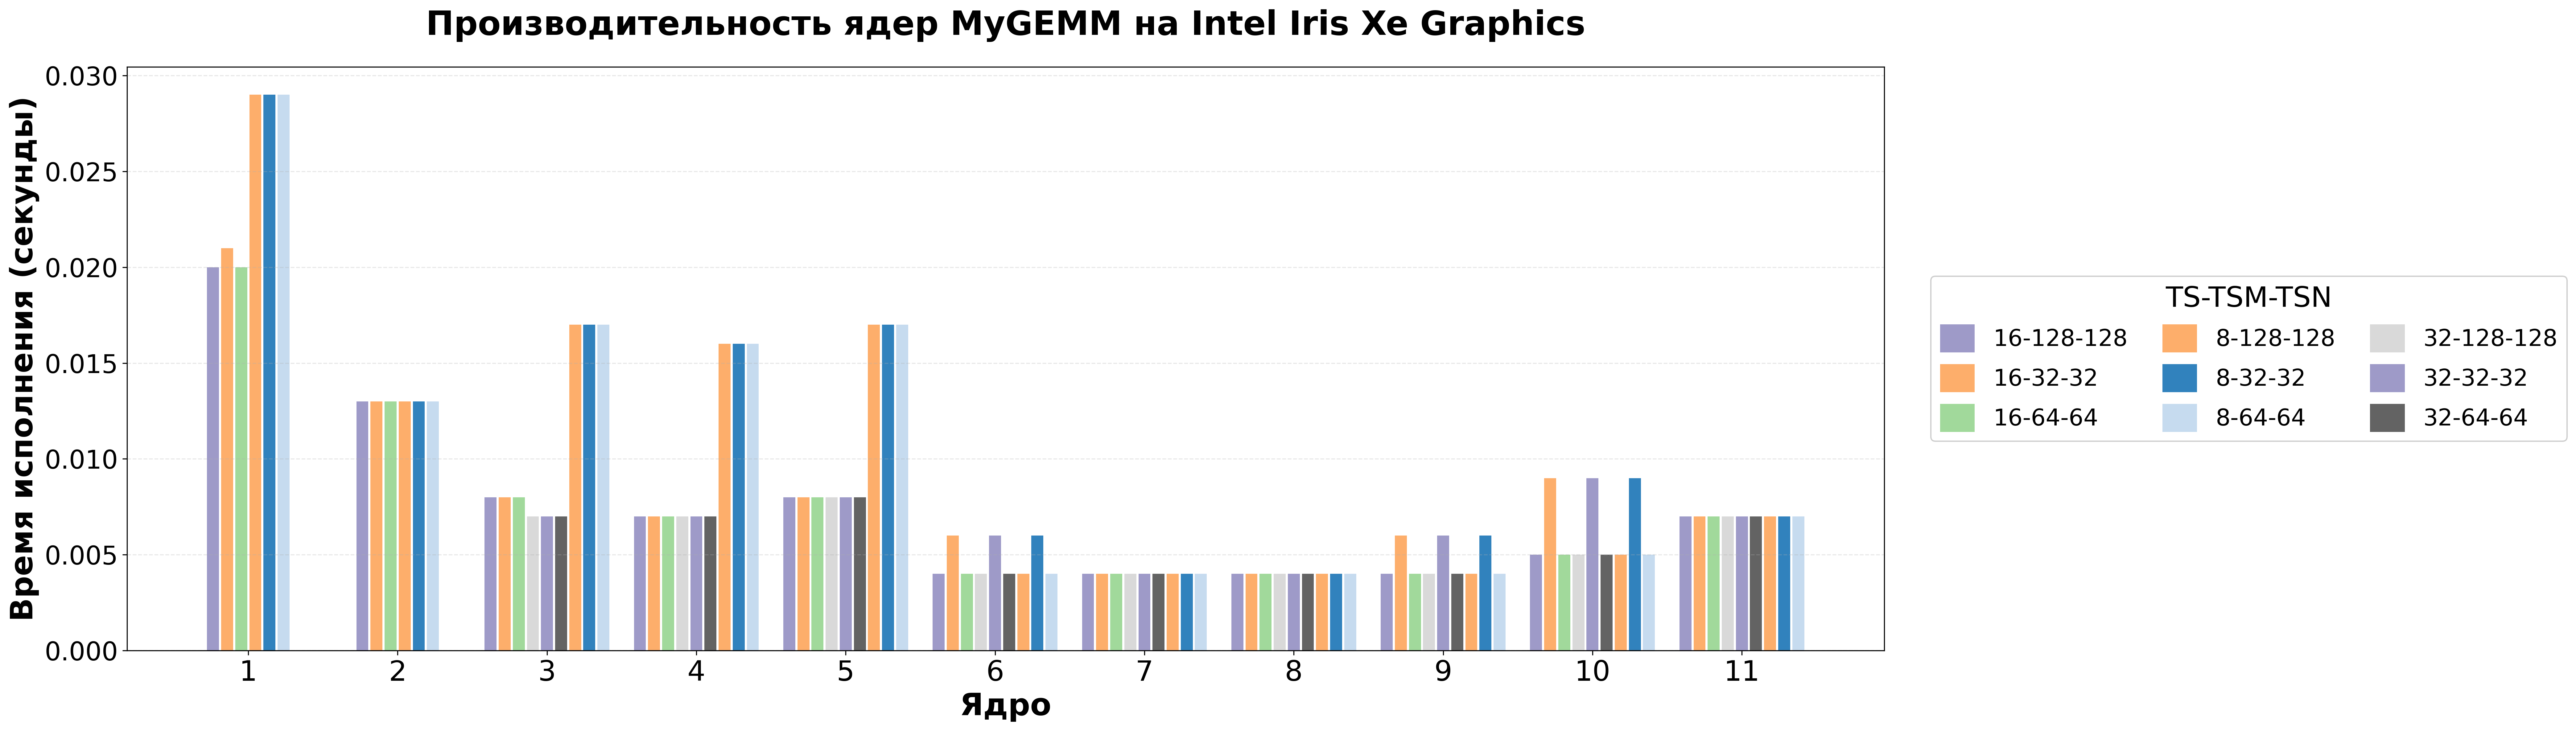
\includegraphics[width=1\textwidth]{figures/intel_xe.png}
\caption{Производительность ядер MyGEMM на платформе Intel Core i9-12900H}
\label{fig:perf_intelxe}
\end{figure}

Ядро 11 показало лучшие результаты на всех RISC-V платформах: 0.32 секунды на Banana Pi (ускорение в 18.4 раза относительно наивной реализации), 0.49 секунды на StarFive (ускорение в 16.1 раза). Ядра 2--5 с использованием локальной памяти дают ускорение в 10--25 раз на RISC-V платформах.

Ядра 6--10 с векторизацией показали низкую производительность: время выполнения 9--11 секунд, что в 10--30 раз медленнее ядер 3--5 и в 600--1000 раз медленнее Intel. Предположительно, это связано с неоптимизированной компиляцией векторных операций \texttt{vload}/\texttt{vstore} в драйверах OpenCL для Imagination Technologies BXE или проблемами выравнивания данных.

На графическом ускорителе Intel Iris Xe наблюдается принципиально иная картина производительности по сравнению с RISC-V платформами. Наилучшие результаты демонстрируют ядра 6–9, использующие векторизацию и продвинутые техники оптимизации памяти, со стабильным временем выполнения 0.004 секунды — что в 1.75–2.5 раза быстрее, чем показывает ядро 11. В отличие от графических ускорителей от Imagination Technologies, где ядро 11 стало оптимальным решением, на Intel оно демонстрирует сравнительно скромные результаты (0.007 секунды), уступая даже более ранним реализациям с использованием локальной памяти (ядра 3–5). 

Это показывает сильную архитектурную зависимость оптимизаций: техники, показывающие хорошую эффективность на одних платформах (регистровый тайлинг для Imagination Technologies), могут давать лишь умеренный прирост на других (Intel), где более эффективными оказываются векторизация и оптимизация доступа к памяти.

\subsection{Тестирование библиотеки CLBlast}

CLBlast устанавливалась и тестировалась с использованием скриптов автоматизации из репозитория matrix-benchmark~\cite{matrix_benchmark_repo}. Параметры сборки и тестирования задавались в конфигурационном файле \texttt{conf.sh}, после чего скрипт \texttt{benchmark.sh} автоматически выполнял загрузку исходного кода, сборку библиотеки и тестирование.

Процедура автоматического тюнинга выполнялась отдельно для каждой платформы с помощью встроенной утилиты по документации CLBlast. После завершения тюнинга библиотека тестировалась повторно с использованием того же скрипта \texttt{benchmark.sh} для оценки влияния оптимизации параметров на производительность.

Результаты тюнинга приведены в таблице~\ref{tab:tuning_effect}.

\begin{table}[h!]
\centering
\caption{Влияние автоматического тюнинга CLBlast (время в мс)}
\label{tab:tuning_effect}
\begin{tabular}{|l|r|r|r|r|}
\hline
\textbf{Платформа} & \textbf{Размер} & \textbf{До тюнинга} & \textbf{После} & \textbf{Изм., \%} \\
\hline
\multirow{3}{*}{StarFive} & 512 & 48.14 & 84.54 & +75.6 \\
 & 1024 & 348.72 & 403.23 & +15.6 \\
 & 7680 & 129438 & 129608 & +0.1 \\
\hline
\multirow{3}{*}{Banana Pi} & 512 & 65.34 & 90.14 & +38.0 \\
 & 1024 & 536.75 & 562.21 & +4.7 \\
 & 7680 & 141445 & 141608 & +0.1 \\
\hline
\multirow{3}{*}{Intel Xe} & 512 & 0.67 & 0.68 & +1.5 \\
 & 1024 & 2.24 & 2.18 & -2.7 \\
 & 7680 & 819.14 & 809.12 & -1.2 \\
\hline
\end{tabular}
\end{table}

На платформах Imagination Technologies тюнинг ухудшает производительность: на матрицах 512×512 замедление составляет 75.6\% для StarFive и 38.0\% для Banana Pi. Для размера 1024×1024 ухудшение меньше --- 15.6\% и 4.7\% соответственно. На больших матрицах (7680×7680) изменения минимальны (около 0.1\%). 

На платформе Intel тюнинг даёт небольшое улучшение: 2.7\% для матриц 1024×1024 и 1.2\% для 7680×7680. 

Автотюнер CLBlast формально соблюдает аппаратные ограничения (не превышает лимит в 32 потока), но его эвристики разработаны для GPU с большими рабочими группами (256--1024 потока). В условиях жёстких ограничений RISC-V эти эвристики работают неэффективно. Параметры по умолчанию, вероятно, были вручную настроены для PowerVR BXE, поэтому они лучше результатов автотюнинга.

Рисунки~\ref{fig:clblast_time} и~\ref{fig:clblast_gflops} иллюстрируют эти результаты. Для операции умноржения матриц среднего размера (до 2048×2048) на платформах Imagination Technologies рекомендуется использовать CLBlast без процедуры автоматического подбора параметров.

\begin{figure}[h!]
\centering
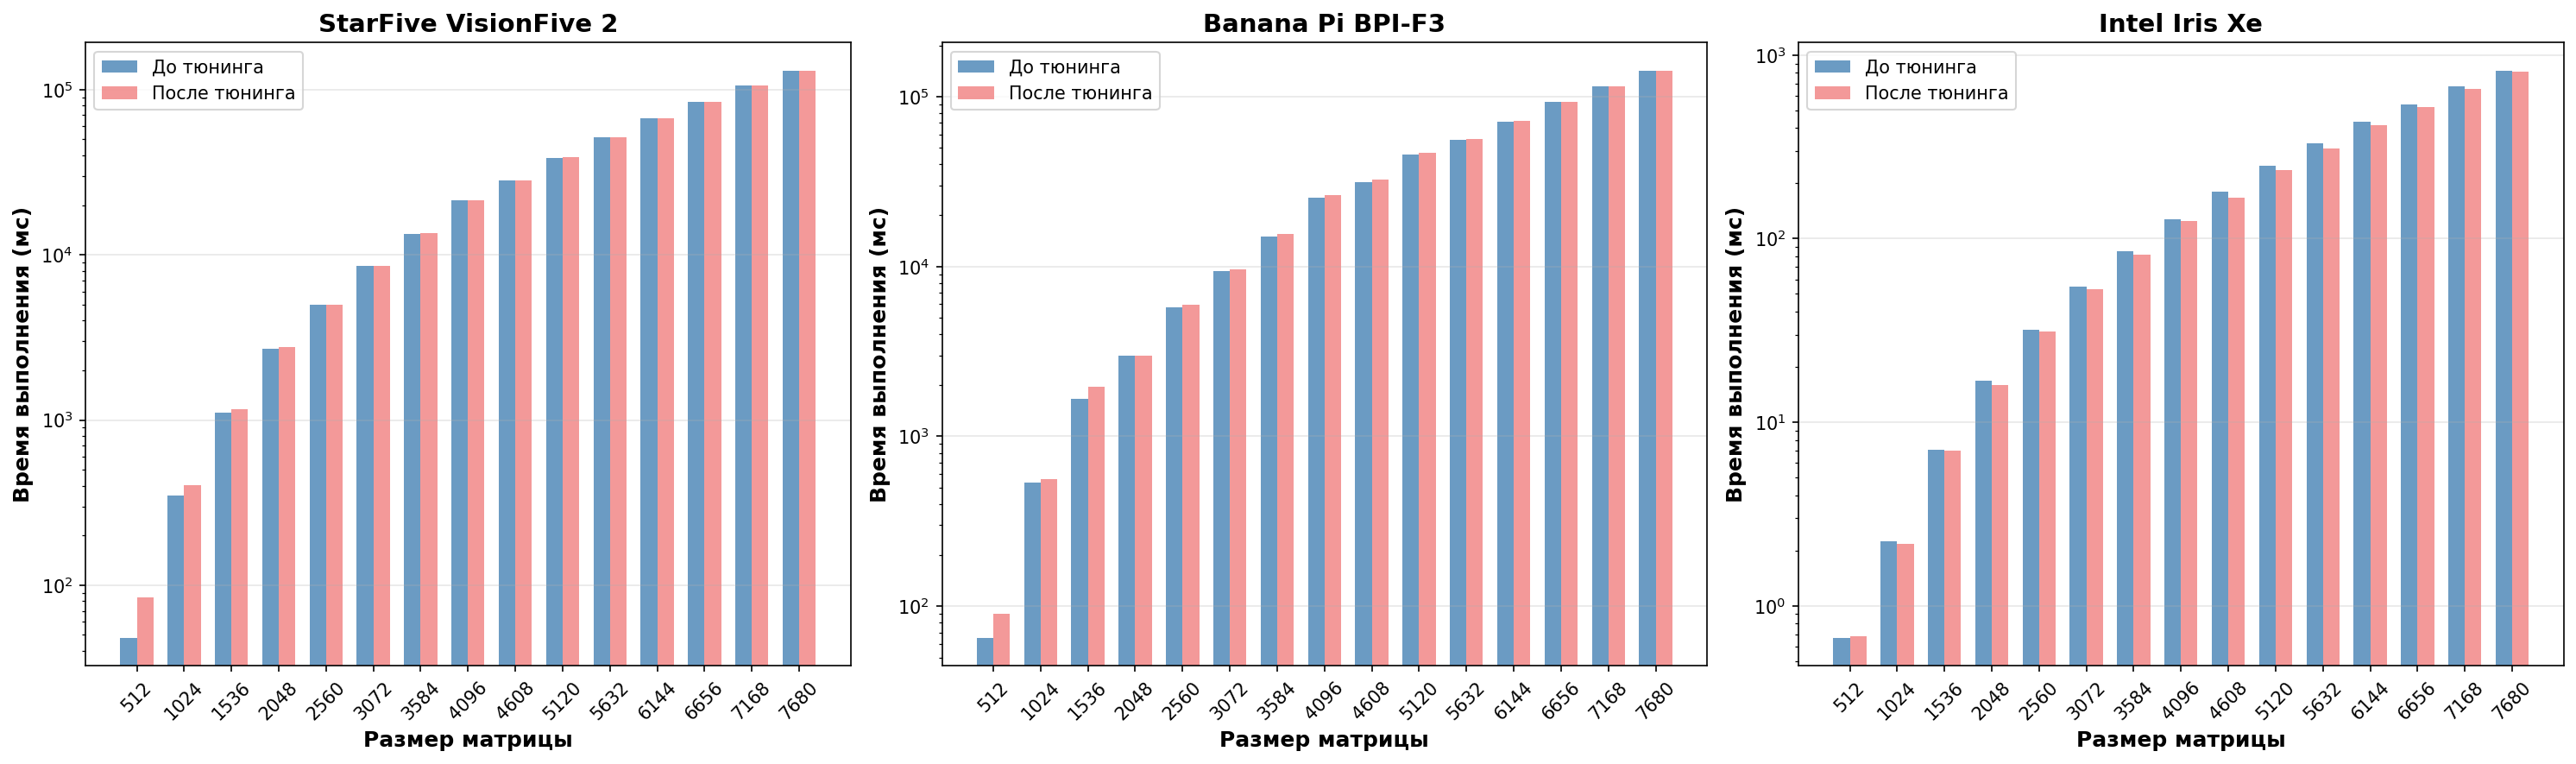
\includegraphics[width=\textwidth]{figures/clblast_time_comparison.png}
\caption{Время выполнения CLBlast до и после тюнинга}
\label{fig:clblast_time}
\end{figure}

\begin{figure}[h!]
\centering
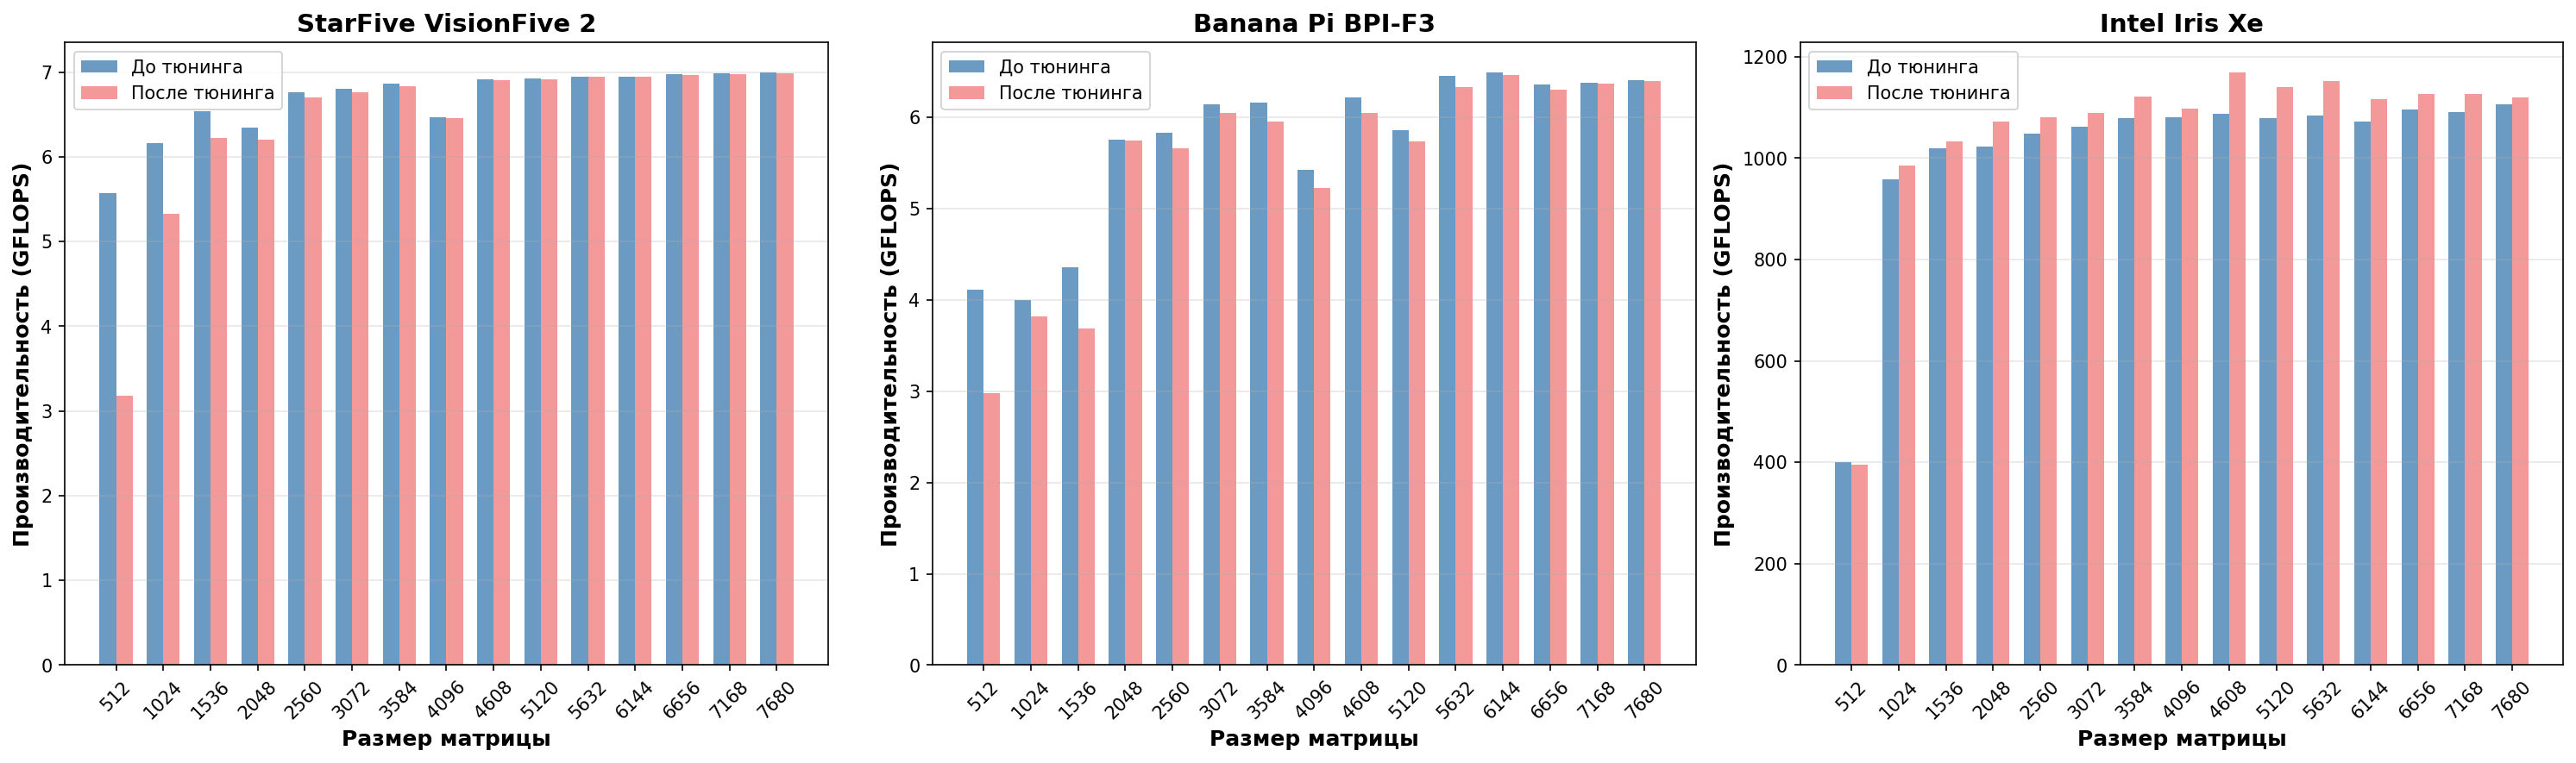
\includegraphics[width=\textwidth]{figures/clblast_gflops.png}
\caption{Производительность CLBlast в GFLOPS}
\label{fig:clblast_gflops}
\end{figure}

\subsection{Сравнение библиотек}

На платформе StarFive библиотека CLBlast с настройками по умолчанию демонстрирует время выполнения 0.349 секунды (6.16 GFLOPS), что примерно на 29\% быстрее, чем лучшее ядро MyGEMM (0.49 секунды). Напротив, на платформе Banana Pi CLBlast (0.537 секунды, 4.01 GFLOPS) уступает лучшему ядру MyGEMM (0.32 секунды) примерно на 68\%. На графическом ускорителе Intel Iris Xe CLBlast показывает лучший результат: его время выполнения (2.24 мс, 959 GFLOPS) более чем в 1.7 раза превосходит лучшие векторизованные ядра MyGEMM (3.8 мс) и почти в 3.2 раза — ядро 11 (7.0 мс). Сравнение производительности для матриц, размер которых 1024 на 1024, представлено на рисунке~\ref{fig:clblast_vs_mygemm}.

Анализ масштабируемости на полном диапазоне размеров матриц подтверждает эти тенденции. На платформах Imagination Technologies CLBlast демонстрируют схожий асимптотический рост времени выполнения, пропорциональный $O(n^3)$. На Intel CLBlast сохраняет значительное преимущество на всех размерах матриц.

\begin{figure}[h!]
\centering
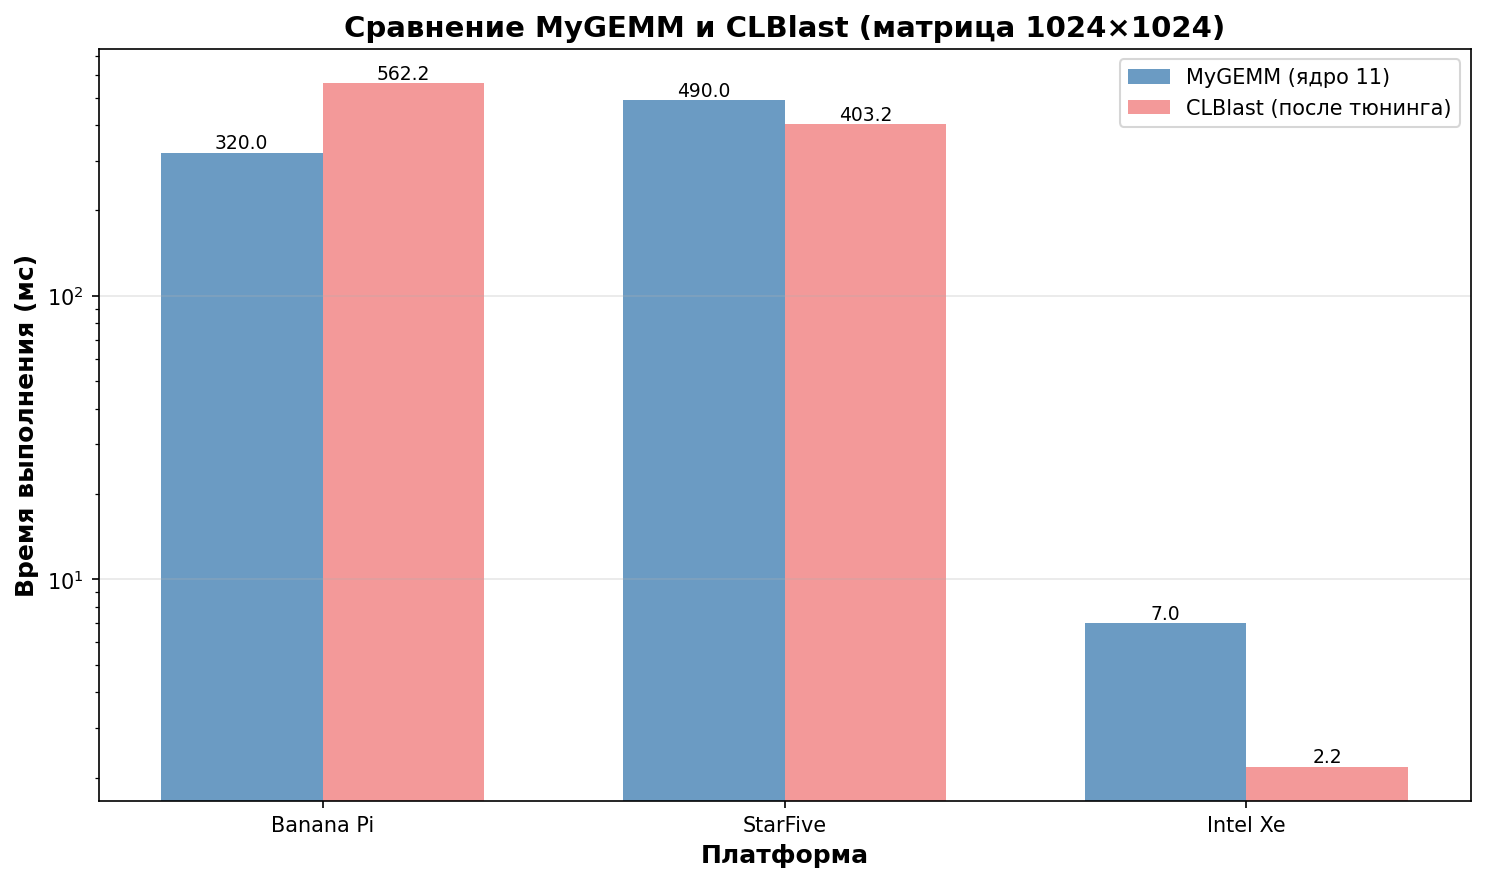
\includegraphics[width=0.8\textwidth]{figures/mygemm_vs_clblast.png}
\caption{Сравнение производительности MyGEMM и CLBlast на матрицах 1024×1024}
\label{fig:clblast_vs_mygemm}
\end{figure}

Автоматический тюнинг CLBlast демонстрирует различную эффективность на разных архитектурах. На платформах Imagination Technologies он приводит к снижению производительности: на StarFive время выполнения увеличилось на 15.6\% (до 0.403 секунды), на Banana Pi — на 4.7\% (до 0.562 секунды).

Обе библиотеки демонстрируют стабильность выполнения со стандартным отклонением менее 2\%. На платформах Imagination Technologies вариативность измерений немного выше, чем на Intel, но остаётся в приемлемых пределах.